\documentclass[final]{beamer}\usepackage[]{graphicx}\usepackage[]{color}
%% maxwidth is the original width if it is less than linewidth
%% otherwise use linewidth (to make sure the graphics do not exceed the margin)
\makeatletter
\def\maxwidth{ %
  \ifdim\Gin@nat@width>\linewidth
    \linewidth
  \else
    \Gin@nat@width
  \fi
}
\makeatother

\definecolor{fgcolor}{rgb}{0.345, 0.345, 0.345}
\newcommand{\hlnum}[1]{\textcolor[rgb]{0.686,0.059,0.569}{#1}}%
\newcommand{\hlstr}[1]{\textcolor[rgb]{0.192,0.494,0.8}{#1}}%
\newcommand{\hlcom}[1]{\textcolor[rgb]{0.678,0.584,0.686}{\textit{#1}}}%
\newcommand{\hlopt}[1]{\textcolor[rgb]{0,0,0}{#1}}%
\newcommand{\hlstd}[1]{\textcolor[rgb]{0.345,0.345,0.345}{#1}}%
\newcommand{\hlkwa}[1]{\textcolor[rgb]{0.161,0.373,0.58}{\textbf{#1}}}%
\newcommand{\hlkwb}[1]{\textcolor[rgb]{0.69,0.353,0.396}{#1}}%
\newcommand{\hlkwc}[1]{\textcolor[rgb]{0.333,0.667,0.333}{#1}}%
\newcommand{\hlkwd}[1]{\textcolor[rgb]{0.737,0.353,0.396}{\textbf{#1}}}%
\let\hlipl\hlkwb

\usepackage{framed}
\makeatletter
\newenvironment{kframe}{%
 \def\at@end@of@kframe{}%
 \ifinner\ifhmode%
  \def\at@end@of@kframe{\end{minipage}}%
  \begin{minipage}{\columnwidth}%
 \fi\fi%
 \def\FrameCommand##1{\hskip\@totalleftmargin \hskip-\fboxsep
 \colorbox{shadecolor}{##1}\hskip-\fboxsep
     % There is no \\@totalrightmargin, so:
     \hskip-\linewidth \hskip-\@totalleftmargin \hskip\columnwidth}%
 \MakeFramed {\advance\hsize-\width
   \@totalleftmargin\z@ \linewidth\hsize
   \@setminipage}}%
 {\par\unskip\endMakeFramed%
 \at@end@of@kframe}
\makeatother

\definecolor{shadecolor}{rgb}{.97, .97, .97}
\definecolor{messagecolor}{rgb}{0, 0, 0}
\definecolor{warningcolor}{rgb}{1, 0, 1}
\definecolor{errorcolor}{rgb}{1, 0, 0}
\newenvironment{knitrout}{}{} % an empty environment to be redefined in TeX

\usepackage{alltt}
\usepackage{grffile}
\mode<presentation>{\usetheme{I6pd2}}

%%%%%%%%%%%%%%%%%%%%%%%%%%%%%%%%%%%%%%%%%%%%%%%%%%%%%%%%%%%%%%%%%%
%%%%%%%%%%%%%%%%%%%%%%%%%%%%%%%%%%%%%%%%%%%%%%%%%%%%%%%%%%%%%%%%%%
%%%%%%%%%%%%%%%%%%%%%%%%%%%%%%%%%%%%%%%%%%%%%%%%%%%%%%%%%%%%%%%%%%
%%%%%%%%%%%%%%%%%%%%%%%%%%%%%%%%%%%%%%%%%%%%%%%%%%%%%%%%%%%%%%%%%%

% =====================================
% Packages
% =====================================

%FORMATTING
\usepackage[normalem]{ulem} 
%for underline, use \uline{ }
%for strikethrough, use \sout{ }

%COLOR
\usepackage{color}
%\usepackage[usenames,dvipsnames]{color}
\usepackage{colortbl} %for table colors

%MATH
\usepackage{amssymb, amsthm, amsmath}
\usepackage{bm} %allows bold greek letters
\usepackage{dsfont} %\mathds{1} for indicator function
\usepackage{breqn} %for breaking up long equations

%PLOTS
\usepackage{graphicx} %for importing graphics files
\usepackage{epstopdf}%for .eps files

%TABLES
\usepackage{bigstrut}
\usepackage{tabularx}
\usepackage{longtable}
\usepackage{multirow}
\usepackage{multicol} % for multicolumn layouts
\usepackage{afterpage}

%VERBATIM
\usepackage{verbatim} %doesnt seem to work with beamer?
\usepackage{fancyvrb} %used for tab spacing in verbatim
\usepackage{listings} %better than fancyvrb in beamer?
\lstset{breaklines=true,basicstyle=\ttfamily\scriptsize} %set font of verbatim thorughout
\def\verb{\lstinline[basicstyle=\ttfamily\small,keywordstyle={}]} %use verb, not lstinline
\def\rcode{\lstinline[basicstyle=\ttfamily\bfseries\small,keywordstyle={}]} 

\newcommand{\balpha}{\mbox{\boldmath $\alpha$} }
\newcommand{\bbeta}{\mbox{\boldmath $\beta$} }
\newcommand{\bdelta}{\mbox{\boldmath $\delta$} }
\newcommand{\bepsilon}{\mbox{\boldmath $\epsilon$} }
\newcommand{\bgamma}{\mbox{\boldmath $\gamma$} }
\newcommand{\blambda}{\mbox{\boldmath $\lambda$} }
\newcommand{\bmu}{\mbox{\boldmath $\mu$} }
\newcommand{\bnu}{\mbox{\boldmath $\nu$} }
\newcommand{\bomega}{\mbox{\boldmath $\omega$} }
\newcommand{\bphi}{\mbox{\boldmath $\phi$} }
\newcommand{\bpsi}{\mbox{\boldmath $\psi$} }
\newcommand{\brho}{\mbox{\boldmath $\rho$} }
\newcommand{\bsigma}{\mbox{\boldmath $\sigma$} }
\newcommand{\btau}{\mbox{\boldmath $\tau$} }
\newcommand{\btheta}{\mbox{\boldmath $\theta$} }
\newcommand{\bupsilon}{\mbox{\boldmath $\upsilon$} }
\newcommand{\bxi}{\mbox{\boldmath $\xi$} }
\newcommand{\bzeta}{\mbox{\boldmath $\zeta$} }
\newcommand{\bDelta}{\mbox{\boldmath $\Delta$} }
\newcommand{\bGamma}{\mbox{\boldmath $\Gamma$} }
\newcommand{\bLambda}{\mbox{\boldmath $\Lambda$} }
\newcommand{\bPhi}{\mbox{\boldmath $\Phi$} }
\newcommand{\bSigma}{\mbox{\boldmath $\Sigma$} }
\newcommand{\bTheta}{\mbox{\boldmath $\Theta$} }

\newcommand{\bfa}{\mbox{\bf a} }
\newcommand{\bfb}{\mbox{\bf b} }
\newcommand{\bfc}{\mbox{\bf c} }
\newcommand{\bfd}{\mbox{\bf d} }
\newcommand{\bfe}{\mbox{\bf e} }
\newcommand{\bff}{\mbox{\bf f} }
\newcommand{\bfg}{\mbox{\bf g} }
\newcommand{\bfh}{\mbox{\bf h} }
\newcommand{\bfi}{\mbox{\bf i} }
\newcommand{\bfj}{\mbox{\bf j} }
\newcommand{\bfk}{\mbox{\bf k} }
\newcommand{\bfl}{\mbox{\bf l} }
\newcommand{\bfm}{\mbox{\bf m} }
\newcommand{\bfn}{\mbox{\bf n} }
\newcommand{\bfo}{\mbox{\bf o} }
\newcommand{\bfp}{\mbox{\bf p} }
\newcommand{\bfq}{\mbox{\bf q} }
\newcommand{\bfr}{\mbox{\bf r} }
\newcommand{\bfs}{\mbox{\bf s} }
\newcommand{\bft}{\mbox{\bf t} }
\newcommand{\bfu}{\mbox{\bf u} }
\newcommand{\bfv}{\mbox{\bf v} }
\newcommand{\bfw}{\mbox{\bf w} }
\newcommand{\bfx}{\mbox{\bf x} }
\newcommand{\bfy}{\mbox{\bf y} }
\newcommand{\bfz}{\mbox{\bf z} }
\newcommand{\bfA}{\mbox{\bf A} }
\newcommand{\bfB}{\mbox{\bf B} }
\newcommand{\bfC}{\mbox{\bf C} }
\newcommand{\bfD}{\mbox{\bf D} }
\newcommand{\bfE}{\mbox{\bf E} }
\newcommand{\bfF}{\mbox{\bf F} }
\newcommand{\bfG}{\mbox{\bf G} }
\newcommand{\bfH}{\mbox{\bf H} }
\newcommand{\bfI}{\mbox{\bf I} }
\newcommand{\bfJ}{\mbox{\bf J} }
\newcommand{\bfK}{\mbox{\bf K} }
\newcommand{\bfL}{\mbox{\bf L} }
\newcommand{\bfM}{\mbox{\bf M} }
\newcommand{\bfN}{\mbox{\bf N} }
\newcommand{\bfO}{\mbox{\bf O} }
\newcommand{\bfP}{\mbox{\bf P} }
\newcommand{\bfQ}{\mbox{\bf Q} }
\newcommand{\bfR}{\mbox{\bf R} }
\newcommand{\bfS}{\mbox{\bf S} }
\newcommand{\bfT}{\mbox{\bf T} }
\newcommand{\bfU}{\mbox{\bf U} }
\newcommand{\bfV}{\mbox{\bf V} }
\newcommand{\bfW}{\mbox{\bf W} }
\newcommand{\bfX}{\mbox{\bf X} }
\newcommand{\bfY}{\mbox{\bf Y} }
\newcommand{\bfZ}{\mbox{\bf Z} }

\newcommand{\iid}{\stackrel{iid}{\sim}}
\newcommand{\indep}{\overset{ind}{\sim}}
\newcommand{\calA}{{\cal A}}
\newcommand{\calB}{{\cal B}}
\newcommand{\calC}{{\cal C}}
\newcommand{\calD}{{\cal D}}
\newcommand{\calF}{{\cal F}}
\newcommand{\calG}{{\cal G}}
\newcommand{\calH}{{\cal H}}
\newcommand{\calI}{{\cal I}}
\newcommand{\calJ}{{\cal J}}
\newcommand{\calK}{{\cal K}}
\newcommand{\calL}{{\cal L}}
\newcommand{\calM}{{\cal M}}
\newcommand{\calN}{{\cal N}}
\newcommand{\calO}{{\cal O}}
\newcommand{\calP}{{\cal P}}
\newcommand{\calQ}{{\cal Q}}
\newcommand{\calR}{{\cal R}}
\newcommand{\calS}{{\cal S}}
\newcommand{\calT}{{\cal T}}
\newcommand{\calX}{{\cal X}}
\newcommand{\argmax}{{\mathop{\rm arg\, max}}}
\newcommand{\argmin}{{\mathop{\rm arg\, min}}}
\newcommand{\Frechet}{ \mbox{Fr$\acute{\mbox{e}}$chet} }
\newcommand{\Matern}{ \mbox{Mat$\acute{\mbox{e}}$rn} }

\newcommand{\bfig}{\begin{figure}}
\newcommand{\efig}{\end{figure}}
\newcommand{\beqx}{\begin{equation*}}
\newcommand{\eeqx}{\end{equation*}}
\newcommand{\beq}{\begin{equation}}
\newcommand{\eeq}{\end{equation}}
\newcommand{\beqa}{\begin{eqnarray}}
\newcommand{\eeqa}{\end{eqnarray}}
\newcommand{\beqax}{\begin{eqnarray*}}
\newcommand{\eeqax}{\end{eqnarray*}}
\newcommand{\beqn}{\begin{dmath}}
\newcommand{\eeqn}{\end{dmath}}
\newcommand{\beqnx}{\begin{dmath*}}
\newcommand{\eeqnx}{\end{dmath*}}

\let\originalleft\left
\let\originalright\right
\renewcommand{\left}{\mathopen{}\mathclose\bgroup\originalleft}
\renewcommand{\right}{\aftergroup\egroup\originalright}

\renewcommand{\colon}{\nobreak\mskip1mu\mathpunct{}\nonscript\mkern-\thinmuskip{:}\mskip6muplus1mu\relax}

\providecommand{\itbf}[1]{\textit{\textbf{#1}}} 
\providecommand{\abs}[1]{\left\lvert#1\right\rvert} 
\providecommand{\norm}[1]{\left\lVert#1\right\rVert}

\providecommand{\paren}[1]{\left(#1\right)} 
\providecommand{\Paren}[1]{\Big(#1\Big)}
\providecommand{\PAREN}[1]{\bigg(#1\bigg)} 
\providecommand{\bracket}[1]{\left[ #1 \right]} 
\providecommand{\Bracket}[1]{\Big[ #1 \Big]} 
\providecommand{\BRACKET}[1]{\bigg[ #1 \bigg]} 
\providecommand{\curlybrace}[1]{\left\{ #1 \right\}} 
\providecommand{\Curlybrace}[1]{\Big\{ #1 \Big\}} 
\providecommand{\CURLYBRACE}[1]{\bigg\{ #1 \bigg\}} 

\newcommand{\cond}{\,\left\vert\vphantom{}\right.}
\newcommand{\Cond}{\,\Big\vert\vphantom{}\Big.}
\newcommand{\COND}{\,\Bigg\vert\vphantom{}\Bigg.}


\newcommand{\Bern}{\mbox{{\sf Bern}}}
\newcommand{\Bernoulli}{\mbox{{\sf Bernoulli}}}
\newcommand{\Beta}{\mbox{{\sf Beta}}}
\newcommand{\Binom}{\mbox{{\sf Binom}}}
\newcommand{\Binomial}{\mbox{{\sf Binomial}}}
\newcommand{\Gam}{\mbox{{\sf Gamma}}}
\newcommand{\InverseGam}{\mbox{{\sf InverseGamma}}}
\newcommand{\GP}{\mbox{{\sf GP}}}
\newcommand{\GPD}{\mbox{{\sf GPD}}}
\newcommand{\MVN}{\mbox{{\sf MVN}}}
\newcommand{\Geom}{\mbox{{\sf Geom}}}
\newcommand{\NB}{\mbox{{\sf NB}}}
\newcommand{\NegBin}{\mbox{{\sf NegBin}}}
\newcommand{\NegativeBinomial}{\mbox{{\sf NegativeBinomial}}}
\newcommand{\Normal}{\mbox{{\sf Normal}}}
\newcommand{\Pois}{\mbox{{\sf Pois}}}
\newcommand{\Poisson}{\mbox{{\sf Poisson}}}
\newcommand{\Unif}{\mbox{{\sf Unif}}}
\newcommand{\Uniform}{\mbox{{\sf Uniform}}}


\newcommand{\Prob}{{\sf Prob}}
\newcommand{\median}{{\mathop{\rm median}}}
\newcommand{\E}{\mathsf{E}}
\newcommand{\V}{\mathsf{V}}
\newcommand{\VAR}{\mathsf{VAR}}
\newcommand{\COV}{\mathsf{COV}}

\newcommand{\Ind}{\mathds{1}}
\newcommand{\zerovect}{\mbox{\bf 0}}
\newcommand{\onesvect}{\mbox{\bf 1}}
\providecommand{\real}[1]{\mathbb{#1}}
\newcommand{\Real}{\mathbb{R}}
\newcommand{\ppd}{\mathcal{P}}
\DeclareMathOperator{\logit}{logit}

%colors
\newcommand{\red}{\textcolor{red}}
\newcommand{\orange}{\textcolor{orange}}
\newcommand{\yellow}{\textcolor{yellow}}
\newcommand{\lime}{\textcolor{lime}}
\newcommand{\green}{\textcolor{green}}
\newcommand{\blue}{\textcolor{blue}}
\newcommand{\cyan}{\textcolor{cyan}}
\newcommand{\teal}{\textcolor{teal}}
\newcommand{\magenta}{\textcolor{magenta}}
\newcommand{\pink}{\textcolor{pink}}
\newcommand{\gray}{\textcolor{gray}}
\newcommand{\lightgray}{\textcolor{lightgray}}
\newcommand{\darkgray}{\textcolor{darkgray}}
\newcommand{\black}{\textcolor{black}}
\newcommand{\white}{\textcolor{white}}

\newcommand{\loyolamaroon}{\textcolor{loyolamaroon}}
\newcommand{\loyolagold}{\textcolor{loyolagold}}

\usepackage[english]{babel}
\usepackage[latin1]{inputenc}
\usepackage{amsmath,amsthm, amssymb, latexsym}


%%%%%%%%%%%%%%%%%%%%%%%%%%%%%%%%%%%%%%%%%%%%%%%%%%%%%%%%%%%%%%%%%%
\usepackage{array,booktabs,tabularx,multirow}
\newcolumntype{Z}{>{\centering\arraybackslash}X} % centered tabularx columns
\newcommand{\pphantom}{\textcolor{ta3aluminium}} % phantom introduces a vertical space in p formatted table columns??!!
\newcommand {\expect}{\mbox{E}}
\newcommand {\var}{\mbox{var}}
\newcommand {\cov}{\mbox{cov}}
\listfiles

%%%%%%%%%%%%%%%%%%%%%%%%%%%%%%%%%%%%%%%%%%%%%%%%%%%%%%%%%%%%%%%%%%
%%%%%%%%%%%%%%%%%%%%%%%%%%%%%%%%%%%%%%%%%%%%%%%%%%%%%%%%%%%%%%%%%%
%%%%%%%%%%%%%%%%%%%%%%%%%%%%%%%%%%%%%%%%%%%%%%%%%%%%%%%%%%%%%%%%%%
%%%%%%%%%%%%%%%%%%%%%%%%%%%%%%%%%%%%%%%%%%%%%%%%%%%%%%%%%%%%%%%%%%
%%%%%%%%%%%%%%%%%%%%%%%%%%%%%%%%%%%%%%%%%%%%%%%%%%%%%%%%%%%%%%%%%%
%%%%%%%%%%%%%%%%%%%%%%%%%%%%%%%%%%%%%%%%%%%%%%%%%%%%%%%%%%%%%%%%%%
%%%%%%%%%%%%%%%%%%%%%%%%%%%%%%%%%%%%%%%%%%%%%%%%%%%%%%%%%%%%%%%%%%
%%%%%%%%%%%%%%%%%%%%%%%%%%%%%%%%%%%%%%%%%%%%%%%%%%%%%%%%%%%%%%%%%%
%%%%%%%%%%%%%%%%%%%%%%%%%%%%%%%%%%%%%%%%%%%%%%%%%%%%%%%%%%%%%%%%%%
%%%%%%%%%%%%%%%%%%%%%%%%%%%%%%%%%%%%%%%%%%%%%%%%%%%%%%%%%%%%%%%%%%
%%%%%%%%%%%%%%%%%%%%%%%%%%%%%%%%%%%%%%%%%%%%%%%%%%%%%%%%%%%%%%%%%%
%%%%%%%%%%%%%%%%%%%%%%%%%%%%%%%%%%%%%%%%%%%%%%%%%%%%%%%%%%%%%%%%%%
%%%%%%%%%%%%%%%%%%%%%%%%%%%%%%%%%%%%%%%%%%%%%%%%%%%%%%%%%%%%%%%%%%
%%%%%%%%%%%%%%%%%%%%%%%%%%%%%%%%%%%%%%%%%%%%%%%%%%%%%%%%%%%%%%%%%%
%%%%%%%%%%%%%%%%%%%%%%%%%%%%%%%%%%%%%%%%%%%%%%%%%%%%%%%%%%%%%%%%%%
%%%%%%%%%%%%%%%%%%%%%%%%%%%%%%%%%%%%%%%%%%%%%%%%%%%%%%%%%%%%%%%%%%
%%%%%%%%%%%%%%%%%%%%%%%%%%%%%%%%%%%%%%%%%%%%%%%%%%%%%%%%%%%%%%%%%%
%%%%%%%%%%%%%%%%%%%%%%%%%%%%%%%%%%%%%%%%%%%%%%%%%%%%%%%%%%%%%%%%%%
%%%%%%%%%%%%%%%%%%%%%%%%%%%%%%%%%%%%%%%%%%%%%%%%%%%%%%%%%%%%%%%%%%
%%%%%%%%%%%%%%%%%%%%%%%%%%%%%%%%%%%%%%%%%%%%%%%%%%%%%%%%%%%%%%%%%%
%%%%%%%%%%%%%%%%%%%%%%%%%%%%%%%%%%%%%%%%%%%%%%%%%%%%%%%%%%%%%%%%%%
%%%%%%%%%%%%%%%%%%%%%%%%%%%%%%%%%%%%%%%%%%%%%%%%%%%%%%%%%%%%%%%%%%
%%%%%%%%%%%%%%%%%%%%%%%%%%%%%%%%%%%%%%%%%%%%%%%%%%%%%%%%%%%%%%%%%%
%%%%%%%%%%%%%%%%%%%%%%%%%%%%%%%%%%%%%%%%%%%%%%%%%%%%%%%%%%%%%%%%%%
%%%%%%%%%%%%%%%%%%%%%%%%%%%%%%%%%%%%%%%%%%%%%%%%%%%%%%%%%%%%%%%%%%
%%%%%%%%%%%%%%%%%%%%%%%%%%%%%%%%%%%%%%%%%%%%%%%%%%%%%%%%%%%%%%%%%%
%%%%%%%%%%%%%%%%%%%%%%%%%%%%%%%%%%%%%%%%%%%%%%%%%%%%%%%%%%%%%%%%%%
%%%%%%%%%%%%%%%%%%%%%%%%%%%%%%%%%%%%%%%%%%%%%%%%%%%%%%%%%%%%%%%%%%
%%%%%%%%%%%%%%%%%%%%%%%%%%%%%%%%%%%%%%%%%%%%%%%%%%%%%%%%%%%%%%%%%%
%%%%%%%%%%%%%%%%%%%%%%%%%%%%%%%%%%%%%%%%%%%%%%%%%%%%%%%%%%%%%%%%%%
%%%%%%%%%%%%%%%%%%%%%%%%%%%%%%%%%%%%%%%%%%%%%%%%%%%%%%%%%%%%%%%%%%
%%%%%%%%%%%%%%%%%%%%%%%%%%%%%%%%%%%%%%%%%%%%%%%%%%%%%%%%%%%%%%%%%%
%%%%%%%%%%%%%%%%%%%%%%%%%%%%%%%%%%%%%%%%%%%%%%%%%%%%%%%%%%%%%%%%%%
%%%%%%%%%%%%%%%%%%%%%%%%%%%%%%%%%%%%%%%%%%%%%%%%%%%%%%%%%%%%%%%%%%
%%%%%%%%%%%%%%%%%%%%%%%%%%%%%%%%%%%%%%%%%%%%%%%%%%%%%%%%%%%%%%%%%%
\graphicspath{{figures/}}
%\usepackage[orientation=landscape,size=custom,width=119,height=89,scale=1.25,debug]{beamerposter}
%\usepackage[orientation=portrait,size=a0,scale=1.25,debug]{beamerposter}
\usepackage[orientation=portrait,size=custom,height=91.44,width=106.68,scale=1.25,debug]{beamerposter}


\newlength{\columnheight}\setlength{\columnheight}{75cm} %****You have to get the height empirically***


%=============================================================%
%======================   HEADER   ===========================%
%=============================================================%

\title{\veryHuge Hurdle Modeling in R Using Bayesian Inference}
\author{\Large Taylor Trippe, \and Dr.~Earvin Balderama}
\institute[LUC]{\large Department of Mathematics \& Statistics, Loyola University Chicago, Chicago, IL, USA }
\date[April 16, 2016]{April 16, 2016} %% I don't know where this goes (earvin)
%=============================================================%
%=======================   HEADER   ==========================%
%=============================================================%
\IfFileExists{upquote.sty}{\usepackage{upquote}}{}
\begin{document}
{

%\usebackgroundtemplate{\includegraphics[width=\paperwidth]{nantucket127-points-terrain.png}} %optional background image
\begin{frame}
\vskip1ex
\begin{columns}
%=============================================================%
\begin{column}{.33\textwidth}
\begin{beamercolorbox}[center,wd=\textwidth]{postercolumn}
\begin{minipage}[T]{.97\textwidth}  % tweaks the width, makes a new \textwidth
\parbox[t][\columnheight]{\textwidth}{ % must be some better way to set the the height, width and textwidth simultaneously
% Since all columns are the same length, it is all nice and tidy.  You have to get the height empirically
%=============================================================%
%=============================================================%
%=============================================================%
%===================   FIRST COLUMN    =======================%
%=============================================================%
%=============================================================%
%=============================================================%

%=============================================================%
\begin{block}{Motivation}
%=============================================================%
	
\begin{itemize}
		\item \textbf{Need:} Effective modeling methods for \red{zero-inflated} and/or \red{over-dispersed} count data.
		\vspace{0.75cm}
    \item \textbf{Goal:} Develop a package of user-friendly functions, utilizing \red{MCMC sampling}, that will best model problematic count data that cannot be fit to any typical distribution.
\end{itemize}
	%\begin{center}
	\vspace{-0.25cm}
	%\end{center}
	
\end{block}
\vfill

%=============================================================%
\begin{block}{Discription}
%=============================================================%
	
\begin{itemize}
	\item \textbf{hurdle(...):} Used to fit single or double-hurdle regression models to count data via \red{Bayesian inference}.
	\begin{center}
		\vspace{-0.5cm}
	\end{center}
	\item \textbf{hurdle\textunderscore control(...):} Various parameters for fitting control of \red{hurdle model} regression.
\end{itemize}
	%\begin{center}
	\vspace{-0.25cm}
	%\end{center}
	
\end{block}
\vfill


%=============================================================%
\begin{block}{Usage}
%=============================================================%

\begin{itemize}
	\item hurdle(y, x = NULL, hurdle = Inf,
	dist = c(``poisson'', ``nb'', ``gpd''),
	dist.2 = c(``none'', ``gpd'', "poisson", ``nb''),\\
	control = hurdle\textunderscore control(...),
	iters = 1000, burn = 500, nthin = 1,
	\\plots = T, progress.bar = T)
\begin{center}
	\vspace{-0.5cm}
\end{center}
	\item hurdle\textunderscore control(a = 1, b = 1, size = 1, beta.prior.mean = 0, \\beta.prior.sd = 1000, beta.tune = 1, pars.tune = 0.2,
	lam.start = 1, \\mu.start = 1,
	sigma.start = 1, xi.start = 1)
\end{itemize}
%\begin{center}
\vspace{-0.25cm}
%\end{center}

\end{block}
\vfill

%=============================================================%
\begin{block}{Arguments}
%=============================================================%


\begin{itemize}
	\item \textbf{hurdle(...)}
	\begin{itemize}
		\item \textbf{y:} numeric response vector.
		\item \textbf{x:} optional numeric predictor matrix.
		\item \textbf{hurdle:} numeric threshold ($\psi$) for `extreme' observations of two-hurdle models. \red{NULL} for one-hurdle models.
		\item \textbf{dist:} character specification of response distribution.
		\item \textbf{dist.2:} character specification of response distribution for `extreme' observations of two-hurdle models.
		\item \textbf{control:} list of parameters for controlling the fitting process, specified by \red{hurdle\textunderscore control()}.
		\item \textbf{iters:} number of iterations for the Markov chain to run. 
		\item \textbf{burn:} numeric burn-in length.
		\item \textbf{nthin:} numeric thinning rate.
		\item \textbf{plots:} logical operator. \red{TRUE} to print plots. 
		\item \textbf{progress.bar:} logical operator. \red{TRUE} to print progress bar. 
	\end{itemize}
	\begin{center}
		\vspace{-0.5cm}
	\end{center}
	\item \textbf{hurdle\textunderscore control(...)}
	\begin{itemize}
		\item \textbf{a:} shape parameter for Gamma($a$, $b$) prior distributions.
		\item \textbf{b:} rate parameter for Gamma($a$, $b$) prior distributions.
		\item \textbf{size:} size ($r$) parameter for NB($r$, $\mu$) likelihood distributions.
		\item \textbf{beta.prior.mean:} mean ($\mu$) for Normal($\mu$, $\sigma^{2}$) prior distributions.
		\item \textbf{beta.prior.sd:} st. deviation ($\sigma$) for Normal($\mu$, $\sigma^{2}$) prior distributions.
		\item \textbf{beta.tune:} MCMC tuning for regression coefficient estimation.
		\item \textbf{pars.tune:} MCMC tuning for parameter estimation.
		\item \textbf{lam.start, mu.start, sigma.start, xi.start:} initial value(s) for parameter(s) of `extreme' observations distribution.
	\end{itemize}
\end{itemize}





\end{block}
%\vfill
}
\end{minipage}
\end{beamercolorbox}
\end{column}
%=============================================================%
\begin{column}{.33\textwidth}
\begin{beamercolorbox}[center,wd=\textwidth]{postercolumn}
\begin{minipage}[T]{.97\textwidth} % tweaks the width, makes a new \textwidth
\parbox[t][\columnheight]{\textwidth}{ % must be some better way to set the the height, width and textwidth simultaneously
% Since all columns are the same length, it is all nice and tidy.  You have to get the height empirically
%=============================================================%
%=============================================================%
%=============================================================%
%===================   SECOND COLUMN   =======================%
%=============================================================%
%=============================================================%
%=============================================================%



%=============================================================%
\begin{block}{Functionality \& Applications}
%=============================================================%
%Left: Median estimate of posterior probability

%Right: Uncertainty interval of estimate.

\begin{minipage}[t][0.1mm]{.5\textwidth}
	
	\vspace{2mm}
 \red{Response} data:
	\begin{itemize}
		\item[] Surveys $\rightarrow$ Boat/aerial continuous-time strip transects.
	\end{itemize}
\vspace{0.7cm}
\red{Environmental} covariates:
	\begin{itemize}
		\item[] $\bfx_1=$ Sea surface  temperature.
		\item[] $\bfx_2=$ Ocean depth.
		\item[] $\bfx_3=$ Chlorophyll-a level.
		\item[] $\bfx_4=$ Distance-to-shore.
	\end{itemize}
\vspace{0.7cm}
\red{Temporal} effects (Fourier basis):
	 \begin{itemize}
	 	\item[] $\bfx_5=sin(\frac{\pi}{6}\cdot \mbox{Month})$.
	 	\item[] $\bfx_6=cos(\frac{\pi}{6}\cdot \mbox{Month})$.
	 \end{itemize}

\end{minipage}

\begin{columns}
	\column{0.5\textwidth}
	\flushright

	\column{0.35\textwidth}\flushleft

	\vspace{-1cm}
	\footnotesize
	\centering
	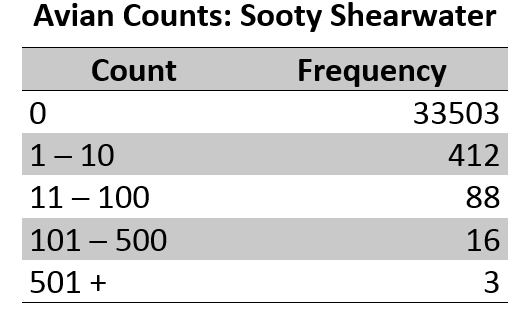
\includegraphics[scale=0.9]{table1.png}\ \
\end{columns}

\vspace{9.1cm}

\begin{minipage}[t][0.01mm]{.97\textwidth}
	\red{Fit} a model to the data in 
\includegraphics[scale=.55]{miscPP.png}\ using \red{hurdlr} package functions:
\end{minipage}

\vspace{1cm}
	
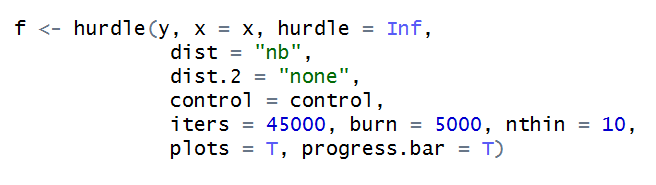
\includegraphics[scale=1.4]{code2.png}\ \

\vspace{0.4cm}

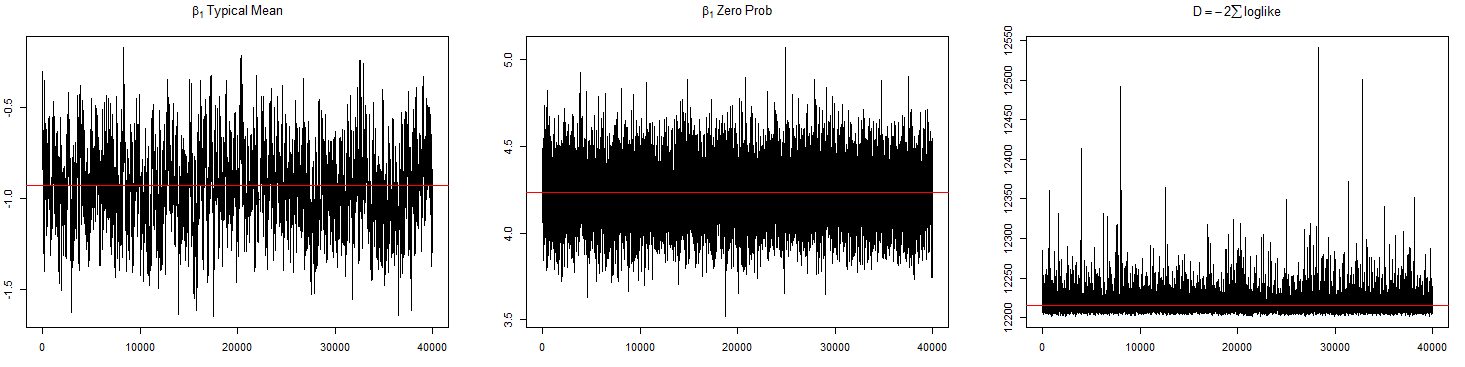
\includegraphics[scale=0.8]{plots2.png}\ \

\vspace{1.2cm}

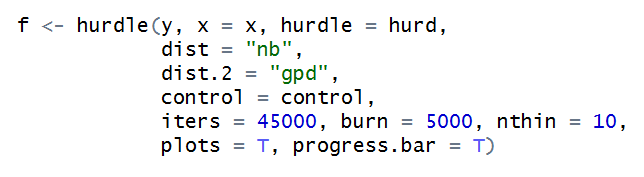
\includegraphics[scale=1.4]{code1.png}\ \

\vspace{0.6cm}

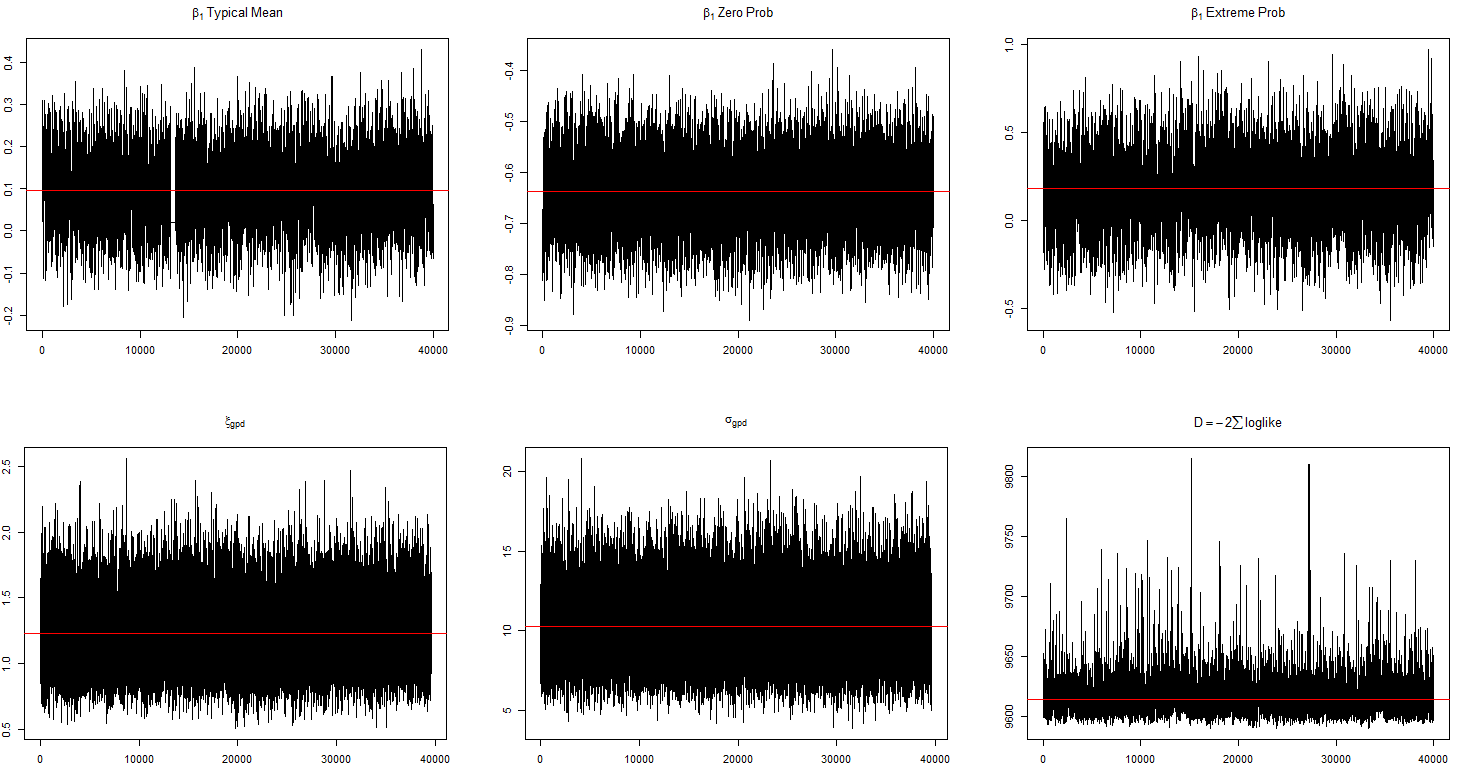
\includegraphics[scale=0.8]{plots4.png}\ \

\vspace{1.2cm}

\begin{minipage}[t][0.1mm]{.97\textwidth}
	
	\red{Compare} Single vs Double Hurdle model:
	\begin{itemize}
		\item[]  $\rightarrow$ Improved convergence of model parameters.
		\item[]  $\rightarrow$ Decrease in deviance (supported by DIC and pD).
		\item[]  $\rightarrow$ Increase in predictive power (based on predictive ordinates PPO\\  \hspace{11mm} and CPO).
	\end{itemize}
	
\end{minipage}

\vspace{7.95cm}





\end{block}
\vfill
}
\end{minipage}
\end{beamercolorbox}
\end{column}
%=============================================================%
\begin{column}{.33\textwidth}
\begin{beamercolorbox}[center,wd=\textwidth]{postercolumn}
\begin{minipage}[T]{.97\textwidth}  % tweaks the width, makes a new \textwidth
\parbox[t][\columnheight]{\textwidth}{ % must be some better way to set the the height, width and textwidth simultaneously
% Since all columns are the same length, it is all nice and tidy.  You have to get the height empirically
%=============================================================%
%=============================================================%
%=============================================================%
%===================   THIRD COLUMN    =======================%
%=============================================================%
%=============================================================%
%=============================================================%



%=============================================================%
\begin{block}{Model}
%=============================================================%
	
	\begin{itemize}
		\item \red{Single-Hurdle modeling} is used to fit \red{zero-inflated} data.
	\end{itemize}
	
	%\item 
	{\bf Likelihood of observing count $y_{i}$:}
	%\end{itemize}
	\begin{equation*}
	f(y_{i} | \blue{\btheta}) = 
	\begin{cases}
		\blue{p_{i}}, &  y_{i}=0,\\
		{[1-p_{i}] \cdot\NB(\blue{\mu_{i}}, r)}, & 1\le y_{ij} < \psi,\\

	\end{cases}
	\end{equation*}
	
	\begin{itemize}
		\item \red{Double-Hurdle modeling} may account for both excessive \red{zero-inflation} and extreme \red{over-dispersion}.
	\end{itemize}

	%\item 
	{\bf Likelihood of observing count $y_{i}$:}
	%\end{itemize}
	\beqx
	f(y_{i} | \blue{\btheta}) = 
	\begin{cases}
		\blue{p_{i}}, &  y_{i}=0,\\
		{[1-p_{i}]\cdot [1-q_{i}] \cdot\NB(\blue{\mu_{i}}, r)}, & 1\le y_{ij} < \psi,\\
		{[1-p_{i}]\cdot \blue{q_{i}}\cdot \GPD(\psi, \sigma, \xi)}, & y_{ij} \ge \psi.
	\end{cases}
	\eeqx
	\begin{itemize}

		\item \red{Negative binomial (NB)} for small, ``typical'' counts.
		\begin{itemize}
			\item Left-truncated at 0 and right-truncated at threshold $\psi$.
			  	\begin{itemize}
						\item Single-hurdle models are truncated only at 0.
						\item ZIP, ZINB, Poisson-hurdle, NB-hurdle distributions are common.
				\end{itemize}
		\end{itemize}
		\item \red{Generalized Pareto (GPD)} for large, right-tail counts.
		\begin{itemize}
			\item GPD density is $>0$ at threshold $\psi$ or above.
		\end{itemize}
		%\end{itemize}
	\end{itemize}
	
	
	
\end{block}
\vfill

%=============================================================%
\begin{block}{Bayesian Regression}
%=============================================================%
	
	
	\begin{itemize}
		

		\item A series of \red{linear regressions} are run to estimate:
		
		\begin{itemize}
			\item[] {$\blue{\itbf{p}}$ \it = \textsf{P}(zero-count)}
			\item[] $\qquad\qquad \logit(\blue{\itbf{p}}) = \bfX\bgamma$
			\item[] {$\blue{\bmu}$ \it = mean of typical-count distribution.}
			\item[] $\qquad\qquad\log(\blue{\bmu}) = \bfX\bbeta$
			\item[] {$\blue{\itbf{q}}$ \it = P(large-count $|$ nonzero-count)}
			\item[] $\qquad\qquad\logit(\blue{\itbf{q}}) = \bfX\bdelta$
			\end{itemize}

		\item A Bayesian approach to linear regression allows for the user to \red{characterize the uncertainty} in the \red{response vector} \textbf{y} through a probability distribution f( \textbf{y}$|$\blue{\btheta}).
		\item Parameters are updated using a home-grown \red{Markov chain Monte Carlo} algorithm utilizing \red{Metropolis} sampling. 
	\end{itemize}
	

\end{block}
\vfill

%=============================================================%
\begin{block}{Current Work \& Future Considerations}
%=============================================================%
\begin{itemize}
	\item Incorporate other distributions; i.e., \red{log-normal} models.
	\item Treat threshold parameter \red{$\psi$} as unknown.
	\item Create similar functions for applying models to zero-inflated (ZIP, ZINP) count distributions.
	\item Increase functionality to allow for \red{hierarchical regression} of \red{nested data}.
	\item Expand on function output to include clean and variable plots, convergence and coverage diagnostics, predictive power, etc.
	\item Release \red{hurdlr} 
\includegraphics[scale=.55]{miscPP.png}\ package to CRAN for public use.
\end{itemize}



\end{block}
\vfill
%=============================================================%
\begin{block}{Acknowledgements}
%=============================================================%


\begin{itemize}
\item Software used: 
\includegraphics[scale=.55]{miscPP.png}\ \ (\url{www.r-project.org}) 
\item Data acquired from: \red{Avian Compendium} (NOAA)
\item Special thanks to Timothy O'Brien and the Loyola University Chicago Department of Mathematics and Statistics.
\end{itemize}



\end{block}





}
\end{minipage}
\end{beamercolorbox}
\end{column}
%%%%%%%%%%%%%%%%%%%%%%%%%%%%%%%%%%%%%%%%%%%%%%%
%%%%%%%%%%%%%%%%%%%%%%%%%%%%%%%%%%%%%%%%%%%%%%%












%++++++++++++++++++++++++++++++++++++++++++++++++++++++++++++++%
%++++++++++++++++++++++++++++++++++++++++++++++++++++++++++++++%
%++++++++++++++++++++++++++++++++++++++++++++++++++++++++++++++%
%++++++++++++++++++++++++++++++++++++++++++++++++++++++++++++++%
%++++++++++++++++++++++++++++++++++++++++++++++++++++++++++++++%
%++++++++++++++++++++++++++++++++++++++++++++++++++++++++++++++%
% end the columns
  \end{columns}
  \vskip1ex
  %\tiny\hfill\textcolor{ta2gray}{Created with \LaTeX \texttt{beamerposter}  \url{http://www-i6.informatik.rwth-aachen.de/~dreuw/latexbeamerposter.php}}

  %\tiny\hfill{Created with \LaTeX \texttt{beamerposter}
  %\url{http://www4.ncsu.edu/$\sim$dmvock/} \hskip1em}
\end{frame}
}
\end{document}


%%%%%%%%%%%%%%%%%%%%%%%%%%%%%%%%%%%%%%%%%%%%%%%%%%%%%%%%%%%%%%%%%%%%%%%%%%%%%%%%%%%%%%%%%%%%%%%%%%%%
%%% Local Variables:
%%% mode: latex
%%% TeX-PDF-mode: t
%%% End:
